\titleformat{\chapter}[display]{\bfseries\centering}{\huge Chapter \thechapter}{1em}{\Huge #1}
\newgeometry{top=3cm, bottom=2.2cm, left=3cm, right=2cm, headsep=1.2cm, footskip=1cm, headheight=0.3cm, textheight=24.5cm, textwidth=16cm}
\onehalfspacing
\pagestyle{fancy}
\fancyhf{}
\renewcommand{\headrulewidth}{0pt}
\lhead{Chapter 5}
\rhead{Results and Discussions}
\cfoot{\thepage}
\chapter{Results and Discussions}

\noindent Results are presented for the application, the scam-text model, the harmful-language rules, auto-scan, the community network, bot detection, the three URL studies, the paired and directed-abuse studies and a comparison with existing systems; research numbers come from the model cards and aggregate result files in the repository \cite{repo}.

\section{Application Results}
\noindent Of the 29 test cases in Table~\ref{tab:tests}, 28 behaved as expected; the exception (TC-25, a genuine UPI debit alert flagged by the text model) is a known limitation discussed in Section~\ref{sec:textres}. Figure~\ref{fig:ui-form}a (Chapter 3) shows the complete result for the parcel-fee scam (TC-24), and Figure~\ref{fig:res-harm} the results for a direct threat and for quoted abuse; in every case the assessments are reported separately, each with its observations, missing checks and a next step.

\begin{figure}[!htbp]
\centering
\begin{minipage}[t]{0.62\linewidth}\centering
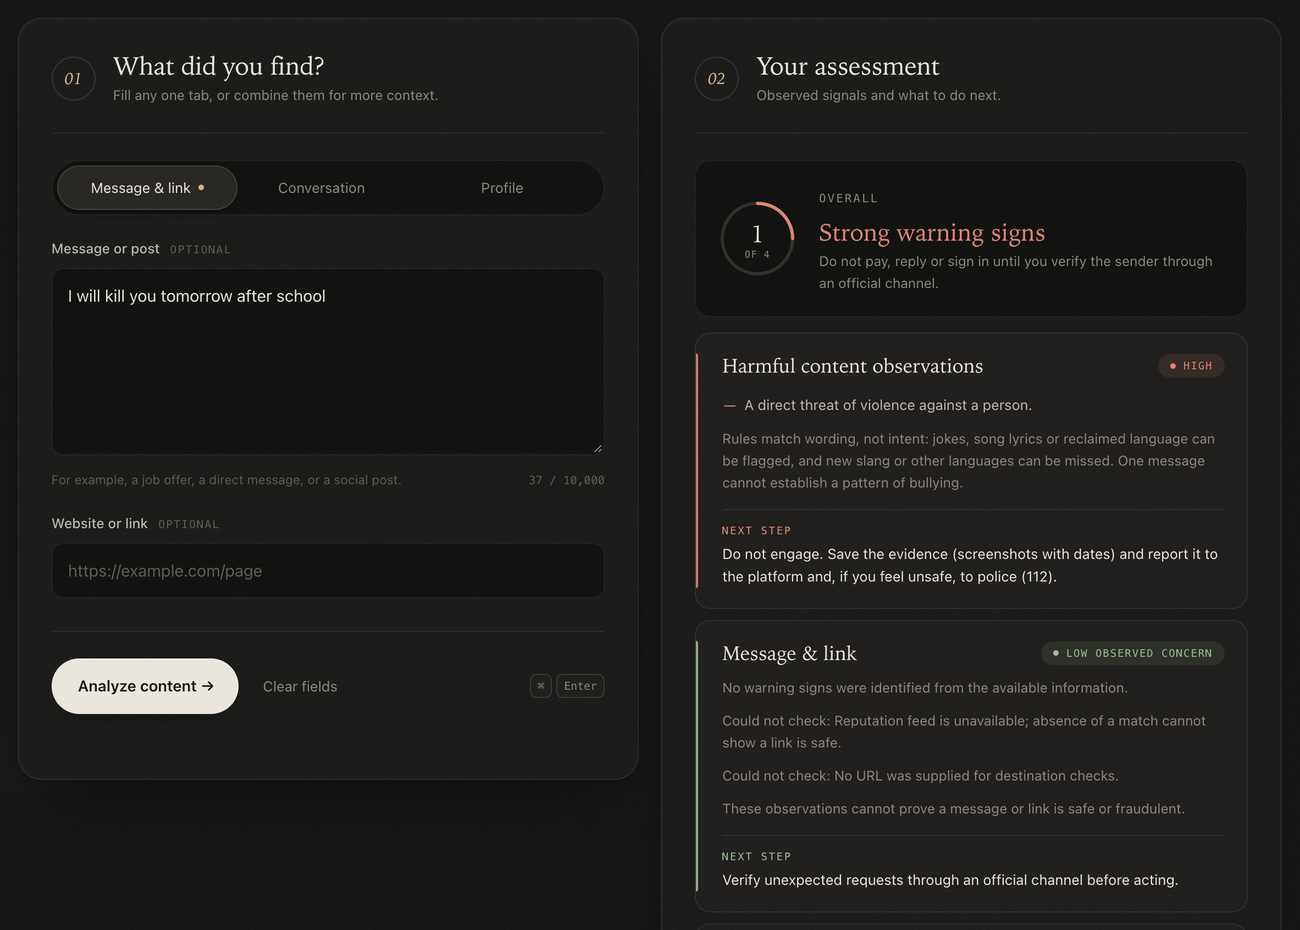
\includegraphics[width=\linewidth]{shots2/check_threat.png}\\[1pt]{\small (a) Direct threat (TC-19): the harm card moves to the top}
\end{minipage}\hfill
\begin{minipage}[t]{0.33\linewidth}\centering
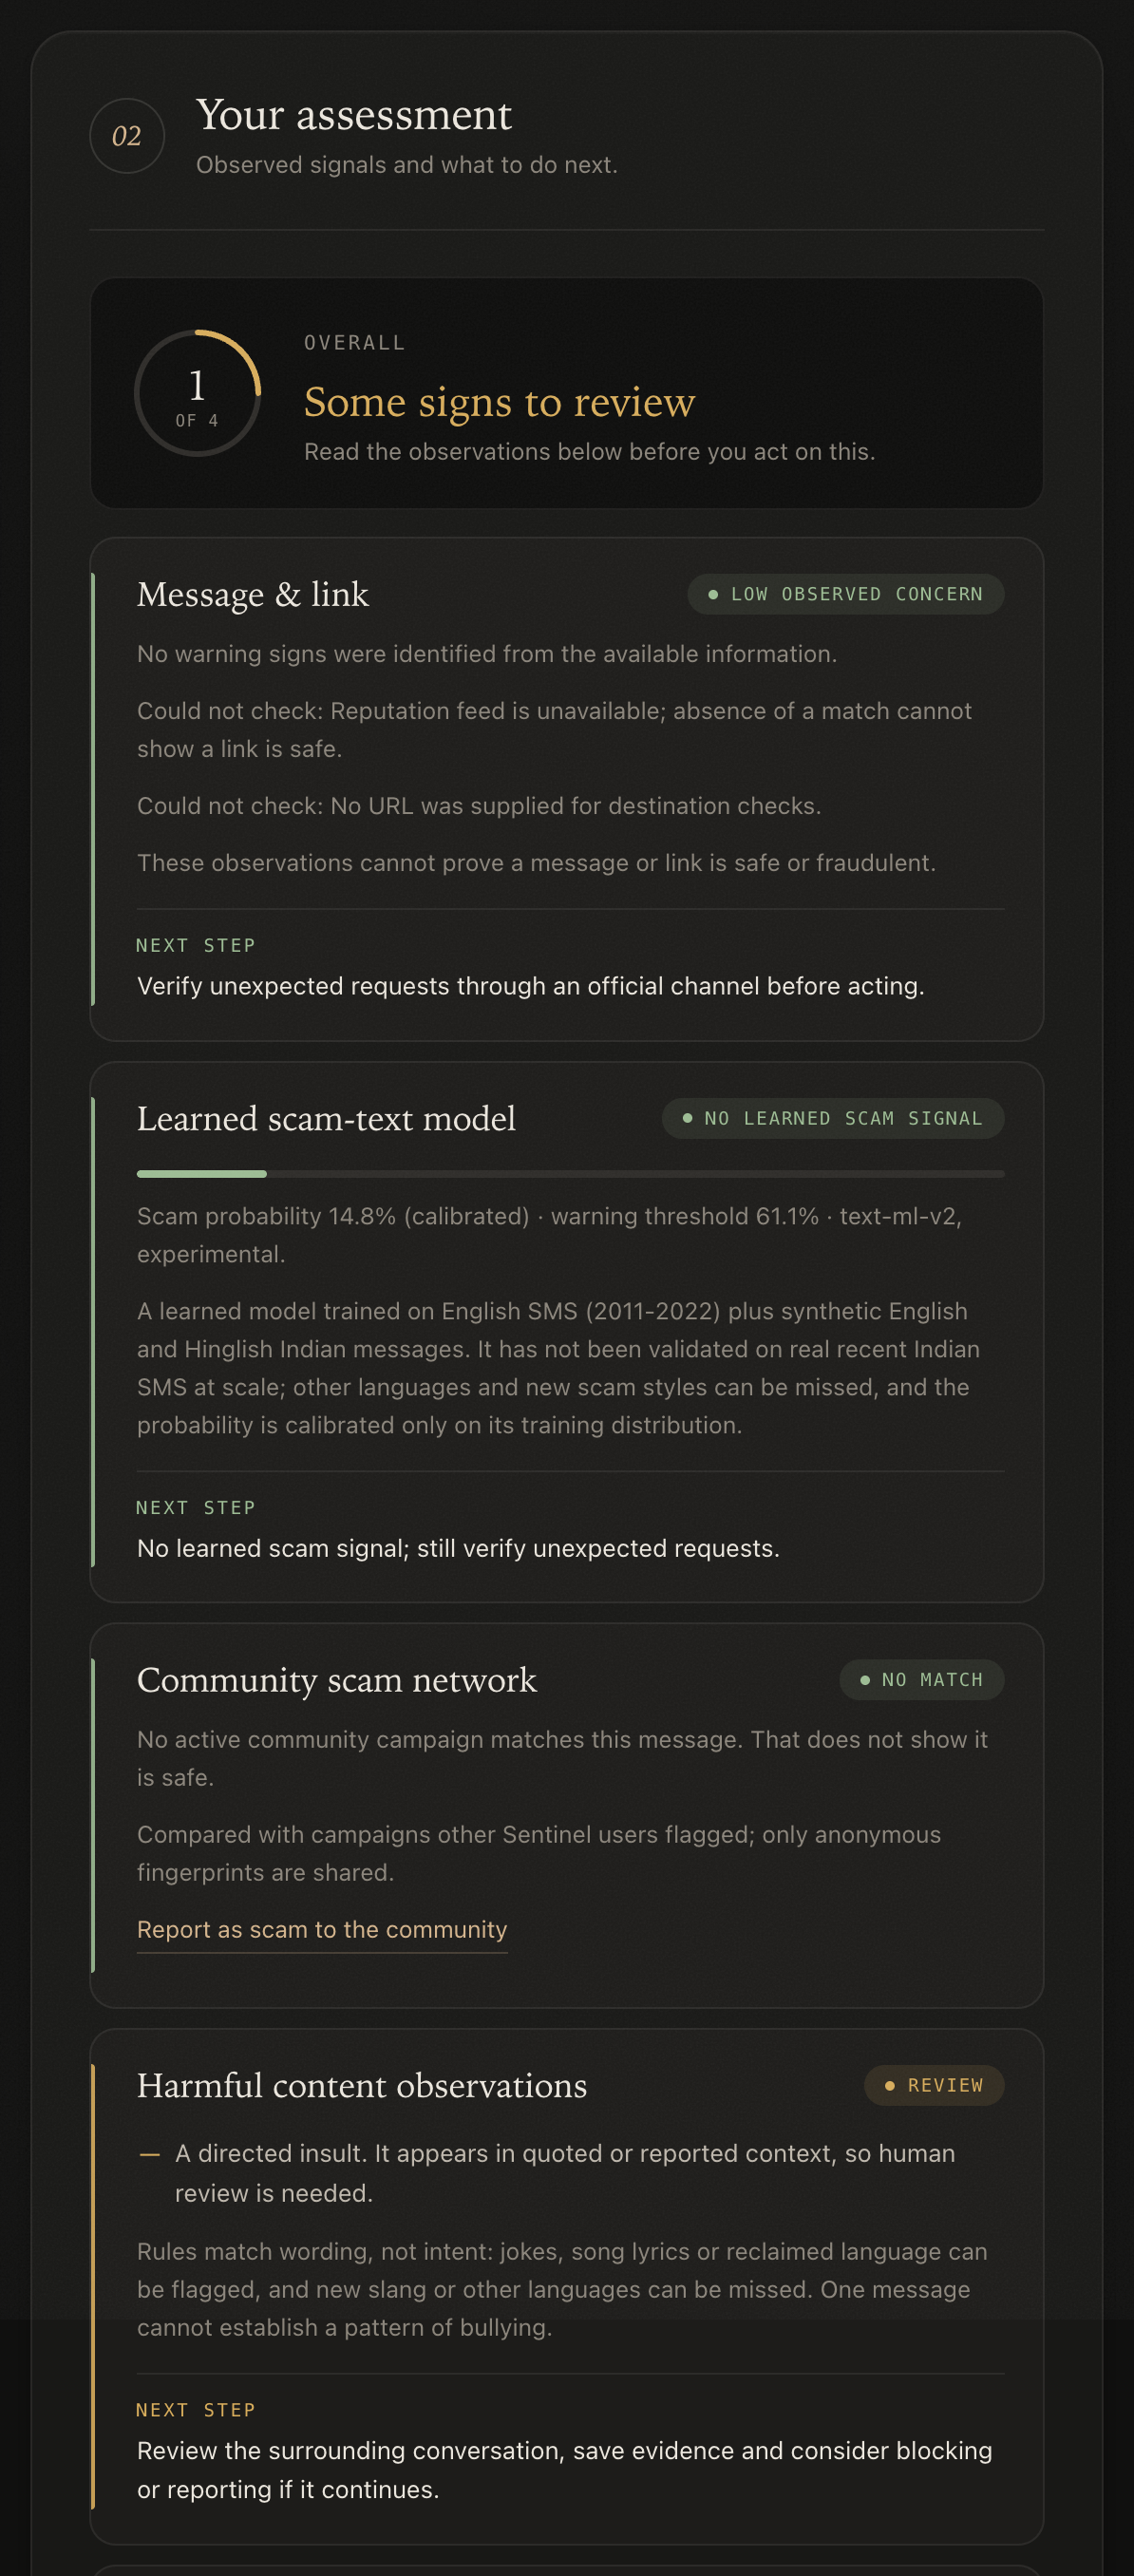
\includegraphics[width=\linewidth]{shots2/check_quoted.png}\\[1pt]{\small (b) Quoted abuse (TC-03): harm card (last) asks for human review}
\end{minipage}
\caption{Harmful-content assessments for a direct threat and for quoted abuse}
\label{fig:res-harm}
\end{figure}

\noindent\textbf{Observations.}
\begin{itemize}
\item The fake internship offer was rated \emph{High} because a payment and OTP request co-occurred with a URL indicator (IP-address host); the result also states that the reputation feed was not loaded, so the link could not be checked against known phishing URLs.
\item The scam-text model did \emph{not} flag the fake internship offer (scam probability 0.56, below 0.611); the rules still rated it High. This is why the model is shown beside the rules and never replaces them.
\item A direct threat (TC-19, and the threat in TC-02) is now rated High with category-specific advice, and the harm card is moved to the top of the page; quoted abuse (TC-03) is lowered to Review and explicitly asks for human review instead of treating the writer as the abuser.
\item The profile check (TC-04) reported all three indicators but kept bot likelihood ``not estimated'', since no validated profile model exists.
\item The ordinary seminar notice (TC-05) received \emph{Low observed concern}, with the reminder that this does not prove the message is safe; in the conversation case (TC-06) the selected third turn was assessed with its two preceding turns as context.
\item The research directed-abuse model is still reported as \emph{Unavailable} in \texttt{/api/health}: no trained harm artifact exists (Section~\ref{sec:cadres}), and live harm detection uses the rule engine instead.
\end{itemize}

\noindent\textbf{Latency.} On the report-preparation machine (a 2-vCPU cloud virtual machine), 180 warm requests to \texttt{/api/analyze} with the TC-01 input took a median of 1.04 ms and a 95th percentile of 1.40 ms end to end, so the rule-based analysis is effectively instantaneous for the user.

\section{Learned Scam-Text Model}\label{sec:textres}
\noindent \textbf{text-ml-v1} was fine-tuned on the Mendeley SMS data (5,790 rows after cleaning, split 70/15/15 by template group so that a resent template never appears in two splits). On the 870-message test split it reached accuracy 0.972 and macro-F1 0.896 (TF-IDF baseline: 0.962 and 0.874); temperature scaling lowered the expected calibration error from 0.0195 to 0.0111, and at its threshold of 0.90 it flagged none of 725 genuine messages with scam recall 0.959. The community-network simulation (Section~\ref{sec:netres}) then exposed a failure the test set could not show: v1 rated genuine Indian transactional messages (bank alerts, OTPs, salary and delivery notices) as scams at 91--99\%, because almost every business-style message in its training data was spam.\\

\noindent \textbf{text-ml-v2} added 2,000 synthetic English and Hinglish Indian rows, kept every v1 row in its v1 split so that the v1 test set is unchanged, chose thresholds on the ONNX outputs, and selected among three candidates on calibration data by a rule fixed in advance. The average of the transformer and the TF-IDF model won (calibration macro-F1 0.933, ham FPR 0.34\%, threshold 0.611). Tables~\ref{tab:text1} and \ref{tab:text2} give the test results.

\begin{table}[H]
\centering
\small
\renewcommand{\arraystretch}{1.15}
\caption{Scam-text model on the unchanged v1 test set (870 Mendeley SMS)}
\label{tab:text1}
\begin{tabular}{|l|c|c|c|c|}
\hline
\textbf{Model} & \textbf{Macro-F1} & \textbf{Scam precision} & \textbf{Scam recall} & \textbf{Genuine flagged} \\ \hline
text-ml-v1 (threshold 0.90) & 0.896 & 1.000 & 0.959 & 0 / 725 \\ \hline
text-ml-v2 (average, 0.611) & 0.897 & 1.000 & 0.966 & 0 / 725 \\ \hline
\end{tabular}
\end{table}

\begin{table}[H]
\centering
\small
\renewcommand{\arraystretch}{1.15}
\caption{Scam-text model on an independent challenge set of 44 messages, written before v2 was trained}
\label{tab:text2}
\begin{tabular}{|l|c|c|}
\hline
\textbf{Model} & \textbf{Genuine wrongly flagged (of 24)} & \textbf{Scams caught (of 20)} \\ \hline
text-ml-v1 & 17 & 14 \\ \hline
v2 transformer alone & 3 & 11 \\ \hline
v2 TF-IDF alone & 4 & 17 \\ \hline
\textbf{text-ml-v2 (average)} & \textbf{2} & \textbf{14} \\ \hline
\end{tabular}
\end{table}

\noindent On the full v2 test set (1,171 rows) the average reached macro-F1 0.925 with precision 1.000, recall 0.983 and no genuine message flagged. The fix therefore cost nothing on the original task while cutting false alarms on genuine Indian messages from 17 of 24 to 2 of 24. Robustness on perturbed scam messages (transformer alone) was 0.980 under leetspeak, 0.976 under Cyrillic look-alike letters and 0.835 under dotted spacing; the ensemble's character n-grams and the community fingerprints partly offset the last. Inference takes about 1.9 ms per message batched on CPU, and the ONNX output matches PyTorch within $3\times10^{-6}$.\\

\noindent\textbf{Limits.} The challenge set is tiny ($n=44$), so its numbers are indicative only. v2 still misses modern conversational scams (``new number, need money'', task-commission and crypto-returns pitches, a ``your son is detained'' message) and still flags some genuine messages: a UPI debit alert scored 0.722 in TC-25. Its added data is synthetic and it has not been validated on real recent Indian SMS; a private evaluation command that prints only counts is provided for that.

\section{Harmful-Language Rule Engine}
\noindent The rule engine replaced a three-phrase rule that flagged only 2 of 11 harmful test sentences. Its unit tests check 12 high-risk sentences (threats, mass violence, self-harm encouragement and risk, sextortion, blackmail, doxxing and dehumanising hate, including Hinglish and disguised forms), 8 directed insults that must go to review (including Hinglish and leetspeak) and 13 benign sentences that must not be flagged (idioms such as ``this movie killed it'', ``kill the process'', ``shoot me an email'', negated threats, everyday Hinglish such as ``mera kutta bahut cute hai''); all pass, as do the quoted-speech, self-harm and advice-priority tests. The application test cases TC-19 to TC-23 confirmed the same behaviour through the API. Because the engine matches wording rather than intent, it can miss new slang and indirect threats; it is explainable, instant and tested, and the learned contextual model (Section~\ref{sec:cadres}) remains the research route to broader coverage.

\section{Auto-Scan Extension}
\noindent The scan endpoint assigned the expected severity to every item in TC-26: a self-harm taunt and the parcel scam \emph{high}, an insult \emph{review} and an ordinary message \emph{none}. On the demonstration chat page (\texttt{/demo}) the scanner marks the job-fee, OTP and bank-login scams and the anonymous insult, and messages added with ``Simulate incoming message'' are scanned as they appear. An idle page scan takes about 190 ms; under heavy CPU load the first scan can exceed the extension's 8-second timeout, after which the scanner pauses and retries. A single weak indicator (one urgent word) is deliberately not marked, to keep ordinary pages free of noise.

\section{Community Scam Network}\label{sec:netres}
\noindent One seeded sweep ran 26 simulations of 10,000 users over 72 hours: 60\% of users share fingerprints, 30 scam campaigns (22 seeded from held-out SMS, 8 invented modern conversational scams) reach 200--2,500 users each and mutate every 6 hours (reworded, then leetspeak, then mixed disguises), and 12 genuine bulk broadcasts reach 500--3,000 users each. Each device runs either the real text-ml-v2 model or a controlled ``rates detector'' whose recall falls with mutation from 96\% to 55\% (assumed values, not measurements).

\begin{table}[H]
\centering
\small
\renewcommand{\arraystretch}{1.15}
\caption{Share of scam deliveries warned, with and without the community network}
\label{tab:net1}
\begin{tabular}{|l|c|c|c|}
\hline
\textbf{Detector on each device} & \textbf{Model alone} & \textbf{Model + network} & \textbf{Caught only by the network} \\ \hline
Rates detector & 78.2\% & 99.7\% & 3,901 \\ \hline
text-ml-v2 (real) & 86.0\% & 93.1\% & 1,280 \\ \hline
text-ml-v1 (real) & 85.3\% & 91.1\% & 1,049 \\ \hline
\end{tabular}
\end{table}

\begin{figure}[H]
\centering
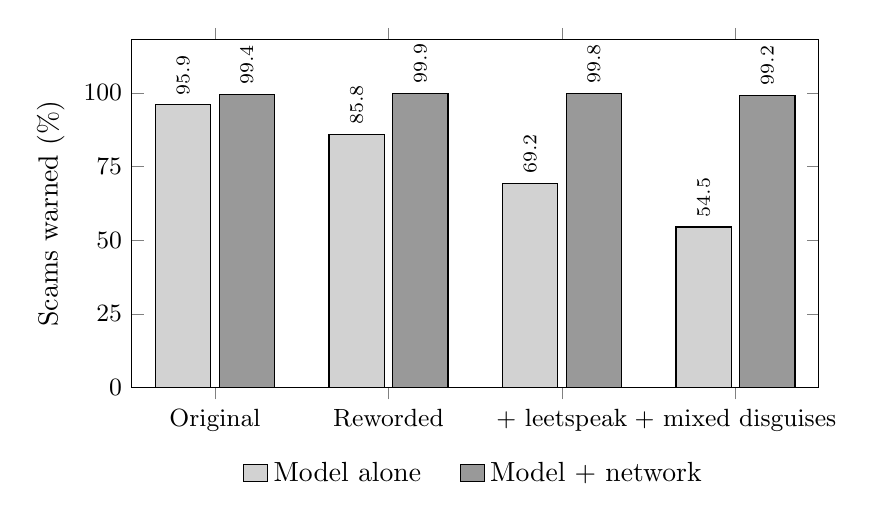
\begin{tikzpicture}
\begin{axis}[ybar=3pt, bar width=20pt, width=0.85\linewidth, height=6cm, ymin=0, ymax=118, ytick={0,25,50,75,100}, ylabel={Scams warned (\%)},
  symbolic x coords={Original,Reworded,+ leetspeak,+ mixed disguises}, xtick=data, enlarge x limits=0.16,
  legend style={at={(0.5,-0.18)}, anchor=north, legend columns=2, draw=none, /tikz/every even column/.append style={column sep=12pt}}, legend image code/.code={\draw[#1] (0cm,-0.1cm) rectangle (0.3cm,0.12cm);},
  nodes near coords, nodes near coords style={font=\scriptsize, rotate=90, anchor=west}, point meta=y,
  every axis plot/.append style={draw=black}, tick label style={font=\small}]
\addplot[fill=gray!35] coordinates {(Original,95.9) (Reworded,85.8) (+ leetspeak,69.2) (+ mixed disguises,54.5)};
\addplot[fill=gray!80] coordinates {(Original,99.4) (Reworded,99.9) (+ leetspeak,99.8) (+ mixed disguises,99.2)};
\legend{Model alone, Model + network}
\end{axis}
\end{tikzpicture}
\caption{Protection by scam mutation level (rates detector)}
\label{fig:netmut}
\end{figure}

\noindent As scammers disguise their messages, each device's own detector gets worse, but the network does not, because the fingerprint undoes the disguises and earlier reports have already published the campaign (Figure~\ref{fig:netmut}). On the eight invented modern scams the real model alone warned only 45.3\%, and the network raised this to 69.6\%, over a third of the gain coming from manual reports by 3\% of users. Larger $k$ delays publication (median 0.95 hours at $k=3$, 1.48 at $k=5$, 3.85 at $k=20$) and costs a little protection. In every run, a search of the full hub database for 5,054 three-word sequences from the simulated messages found none.\\

\begin{table}[H]
\centering
\small
\renewcommand{\arraystretch}{1.15}
\caption{Genuine bulk messages wrongly warned by the network (rates detector)}
\label{tab:net2}
\begin{tabular}{|l|c|}
\hline
\textbf{Configuration} & \textbf{Genuine messages wrongly warned} \\ \hline
No defences, no attackers & 54.4\% \\ \hline
Allowlist and newcomer weight, no disputes & 36.7\% \\ \hline
All defences (allowlist, newcomer weight, disputes) & 2.4\% \\ \hline
All defences, every sender verified & 0.0\% \\ \hline
\end{tabular}
\end{table}

\noindent The main finding is that the largest risk is not attackers but honest false positives at scale: a genuine message sent to 3,000 people at a 0.4\% false-positive rate already gives about 7 reports, more than $k=5$. Only the verified-sender allowlist together with recipient disputes kept wrong campaigns rare (Table~\ref{tab:net2}). With up to 50 attackers poisoning an unregistered sender, disputes withdrew the campaign every time, though more attackers kept it alive longer (6.0\% wrongly warned at 50 attackers). Finally, the network multiplies the quality of its users' detectors: with v1 on every device, 54.1\% of genuine bulk messages were wrongly warned even with all defences; with v2, 0.0\%. This result is what led to text-ml-v2. The simulation's spread curves, mutation operators and user behaviour are assumptions, the modern scams are invented, and the hub is a loopback prototype without production authentication.

\section{Bot-Account Detection}
\noindent\textbf{Profile model (bot-ml-v1).} Thirteen Bot Repository datasets (111,168 Twitter accounts) were used, with 16 profile features obtainable at analysis time; ``verified'' and the default-picture flag were excluded because they reveal the source dataset. Gradient boosting was selected by a rule fixed in advance and reached AUC 0.967 on a mixed, same-distribution split, but the release gate required AUC $\ge$ 0.80 on \emph{every} held-out dataset (Table~\ref{tab:bot1}).

\begin{table}[H]
\centering
\small
\renewcommand{\arraystretch}{1.12}
\caption{Profile model: ROC AUC on each held-out (unseen) dataset}
\label{tab:bot1}
\begin{tabular}{|l|c|c|c|}
\hline
\textbf{Held-out dataset (accounts)} & \textbf{Heuristic} & \textbf{Gradient boosting} & \textbf{Logistic regression} \\ \hline
gilani-2017 (2,465) & 0.510 & 0.600 & 0.577 \\ \hline
cresci-rtbust-2019 (693) & 0.478 & 0.664 & 0.716 \\ \hline
cresci-stock-2018 (13,275) & 0.539 & 0.618 & 0.651 \\ \hline
midterm-2018 (50,534) & 0.978 & 0.821 & 0.979 \\ \hline
botometer-feedback-2019 (509) & 0.624 & 0.785 & 0.756 \\ \hline
cresci-2015 (5,301) & 0.945 & 0.937 & 0.920 \\ \hline
cresci-2017 (11,012) & 0.780 & 0.706 & 0.857 \\ \hline
\textbf{Mean} & 0.693 & 0.733 & 0.779 \\ \hline
\end{tabular}
\end{table}

\noindent The worst held-out AUC was 0.600 (gilani-2017), so the gate failed and the model's estimate is withheld from the application (shown only in an explicit research mode). High scores on mixed data overstate real-world accuracy, and profile metadata alone cannot separate bots whose profiles look human \cite{yang2020}.\\

\noindent\textbf{Activity model (bot-ml-activity-v1).} Only cresci-2015 and cresci-2017 include post histories. Each account's latest 100 posts were turned into 17 activity and content features by the same functions Sentinel applies to uploaded posts, plus the 16 profile features (10,422 accounts). The protocol held out each bot family in turn for model selection and kept a cross-dataset check (train on one cresci dataset, test on the other) untouched until the end.

\begin{table}[H]
\centering
\small
\renewcommand{\arraystretch}{1.12}
\caption{Activity model: ROC AUC on held-out bot families and datasets}
\label{tab:bot2}
\begin{tabular}{|l|c|c|c|}
\hline
\textbf{Held-out fold} & \textbf{Heuristic} & \textbf{Gradient boosting} & \textbf{Logistic regression} \\ \hline
Fake followers & 0.700 & 0.949 & 0.946 \\ \hline
Social spambots 1 & 0.157 & 0.981 & 0.822 \\ \hline
Social spambots 2 & 0.956 & 0.991 & 0.992 \\ \hline
Social spambots 3 & 0.893 & 0.991 & 0.935 \\ \hline
Traditional spambots & 0.537 & 0.995 & 0.995 \\ \hline
cresci-2015 $\rightarrow$ cresci-2017 & 0.720 & 0.849 & 0.938 \\ \hline
cresci-2017 $\rightarrow$ cresci-2015 & 0.720 & 0.884 & 0.956 \\ \hline
\end{tabular}
\end{table}

\noindent Gradient boosting was selected (worst bot-family AUC 0.949 against 0.822); its worst fold over both protocols was 0.849 and its calibration error 0.007, so the gate passed and the model is shown as a separate probability line for X accounts with at least 20 timed posts. Activity patterns generalise far better than profile metadata: the social spambots built to look human were caught at AUC 0.981 without being seen in training, while the hand-set heuristic scored 0.157 on them, worse than chance. Logistic regression did better on the cross-dataset check; the pre-set selection rule is reported rather than changed after the fact. The training data covers Twitter accounts from about 2009--2017, so newer bots and other platforms are out of distribution. In the application, the heuristic separated the uploaded automated and human-like test accounts clearly (82/100 against 4/100, TC-28).

\section{URL Study 1: PhiUSIIL Benchmark}\label{sec:v1res}
\noindent The PhiUSIIL data were split by whole domain groups into 164,741 training URLs and 23,534 URLs each for validation, calibration and test (seed 42). Ten configurations were fitted (six character TF-IDF + logistic regression and four lexical gradient boosting). The validation-selected model was character TF-IDF + logistic regression with $C=10$, no class weighting and 50,000 features. Table~\ref{tab:v1} reports the frozen test results on 23,534 URLs from 19,729 unseen domain groups.

\begin{table}[H]
\centering
\small
\renewcommand{\arraystretch}{1.15}
\caption{URL-v1 test results (\%) on 23,534 domain-held-out URLs}
\label{tab:v1}
\begin{tabular}{|l|c|c|c|c|}
\hline
\textbf{Method} & \textbf{Precision} & \textbf{Recall} & \textbf{F1} & \textbf{FPR} \\ \hline
Char TF-IDF + LR (selected) & 94.48 & 99.80 & 97.07 & 4.35 \\ \hline
Lexical HGB & 94.31 & 99.38 & 96.78 & 4.47 \\ \hline
Phase-0 URL rules & 78.15 & 7.65 & 13.94 & 1.59 \\ \hline
95\% interval (selected) & 93.47--95.44 & 99.71--99.89 & 96.51--97.59 & 4.00--4.73 \\ \hline
\end{tabular}
\end{table}



\begin{figure}[!htbp]
\centering
\begin{minipage}{0.41\linewidth}\centering
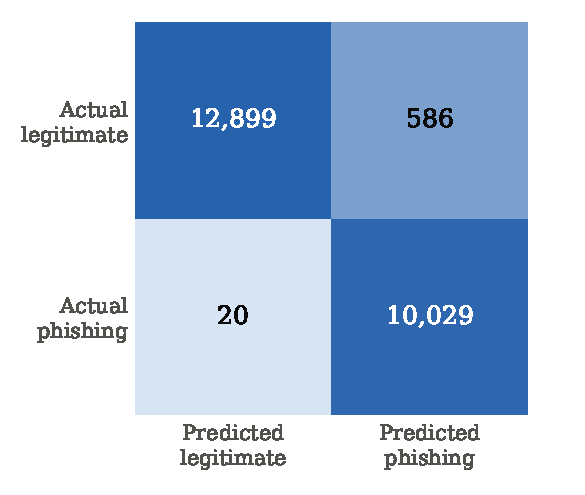
\includegraphics[width=\linewidth]{charts/c2_v1_confusion.pdf}
\end{minipage}\hfill
\begin{minipage}{0.45\linewidth}\centering
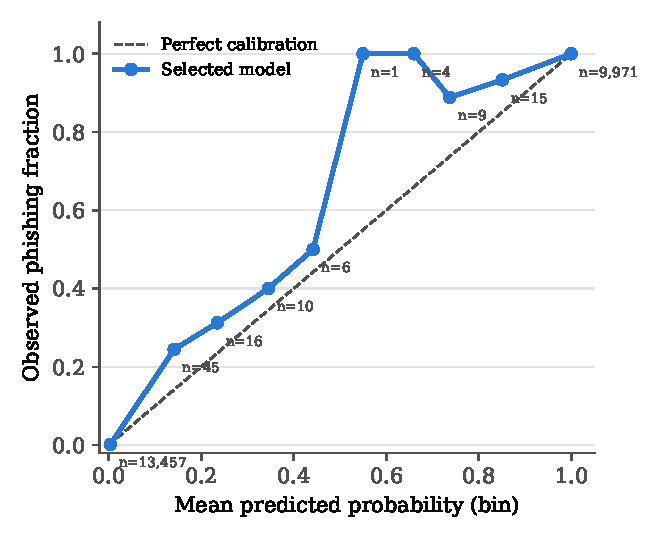
\includegraphics[width=\linewidth]{charts/c3_v1_reliability.pdf}
\end{minipage}
\caption{Confusion matrix (left) and reliability diagram after calibration (right) for the selected URL-v1 model}
\label{fig:v1cm}
\end{figure}

\noindent The selected model made 586 false positives and 20 false negatives. Its average precision was 0.9994. After sigmoid calibration on the separate calibration partition, the test Brier score was 0.0020 and the expected calibration error 0.0015; Figure~\ref{fig:v1cm} shows that almost all URLs receive probabilities near 0 or 1. The ten fits used at most 0.92 GiB of memory (493 seconds in total), and prediction took 6.75 ms (median) and 9.09 ms (95th percentile) per URL on CPU after a 1.15 s cold start.\\

\noindent\textbf{Why this result is not deployed.} An audit of the source (Figure~\ref{fig:format}) found that every one of the 134,850 legitimate URLs is an HTTPS, \texttt{www}-prefixed home page with an empty path and no query, while phishing URLs have varied formats. The model can therefore partly learn the collection format. A separate check flagged \texttt{https://example.org/} and an official Python documentation page as phishing. Moreover, at a realistic prevalence the measured rates give low precision (Section~\ref{sec:metrics}): if only 0.1\% of URLs were phishing, about 2.25\% of warnings would be correct. The model was therefore kept research-only.

\begin{figure}[!htbp]
\centering
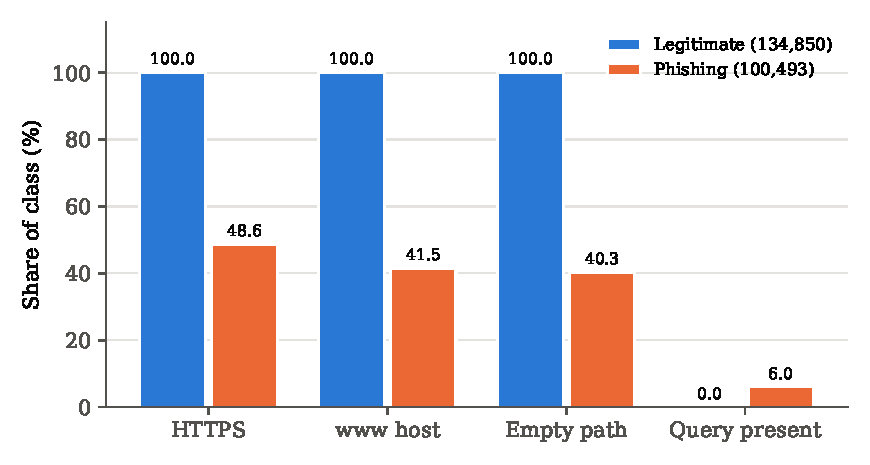
\includegraphics[width=0.62\linewidth]{charts/c8_format_audit.pdf}
\caption{URL format audit of the PhiUSIIL source by class}
\label{fig:format}
\end{figure}



\section{URL Study 2: PhreshPhish Data Gate}
\noindent To obtain more varied legitimate URLs, URL-v2 imported 666,315 PhreshPhish observations and retained 660,130 canonical URLs. Before training, the frozen 200,000-row development set was checked against predeclared format-coverage gates for legitimate URLs: non-root paths (63,850 observed, 100 required) and non-\texttt{www} hosts (34,320 observed, 100 required) passed, but only 6 legitimate URLs with a query string were present against a minimum of 30, so training was stopped. No v2 model or accuracy is claimed; this is a valid negative result that prevented another format-biased model.

\section{URL Study 3: PhreshPhish and Mendeley}
\noindent URL-v3 added the Mendeley web-page phishing dataset, audited 671,521 canonical URLs jointly, passed all coverage gates and trained ten configurations on a 160,000-row partition (peak fit memory about 1.19 GiB). The validation-selected model was character TF-IDF + logistic regression with $C=10$ and balanced class weights. It was evaluated once on two frozen tracks: a primary PhreshPhish track (166,369 URLs, 78,202 components) and a supplemental Mendeley track (4,348 URLs, 3,265 components) that is group-held-out but from a source also used in development.

\begin{table}[H]
\centering
\small
\renewcommand{\arraystretch}{1.15}
\caption{URL-v3 results (\%) at the 5\% validation-FPR operating point}
\label{tab:v3}
\begin{tabular}{|l|l|c|c|c|c|}
\hline
\textbf{Track} & \textbf{Method} & \textbf{Precision} & \textbf{Recall} & \textbf{F1} & \textbf{FPR} \\ \hline
\multirow{4}{*}{\makecell[l]{Primary\\(166,369)}} & Char TF-IDF + LR (selected) & 93.19 & 92.23 & 92.71 & 5.76 \\ \cline{2-6}
 & Lexical HGB & 95.79 & 80.54 & 87.51 & 3.02 \\ \cline{2-6}
 & Format-only control & 98.88 & 32.25 & 48.63 & 0.31 \\ \cline{2-6}
 & Phase-0 URL rules & 84.67 & 7.15 & 13.19 & 1.11 \\ \hline
\multirow{4}{*}{\makecell[l]{Supplemental\\(4,348)}} & Char TF-IDF + LR (selected) & 82.96 & 84.83 & 83.88 & 22.39 \\ \cline{2-6}
 & Lexical HGB & 73.21 & 65.60 & 69.20 & 30.85 \\ \cline{2-6}
 & Format-only control & 78.60 & 61.88 & 69.24 & 21.65 \\ \cline{2-6}
 & Phase-0 URL rules & 98.58 & 14.23 & 24.87 & 0.26 \\ \hline
\end{tabular}
\end{table}

\begin{figure}[!htbp]
\centering
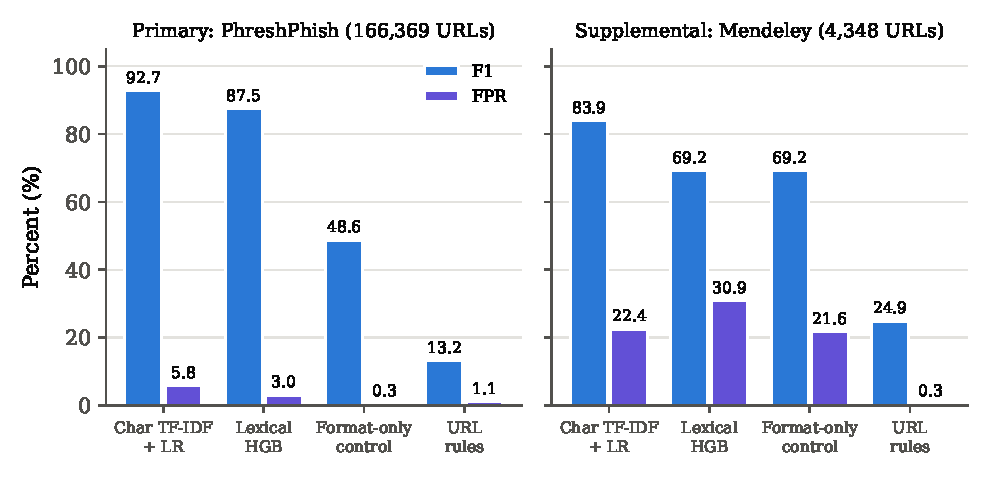
\includegraphics[width=0.72\linewidth]{charts/c5_v3_tracks.pdf}
\caption{URL-v3 F1 and false-positive rate on the primary and supplemental tracks}
\label{fig:v3}
\end{figure}

\noindent On the primary track the selected model kept a strong F1 of 92.71\%, clearly better than the format-only control (48.63\%) and the rules (13.19\%). On the supplemental track its FPR rose to 22.39\%, and legitimate URLs with query strings were wrongly flagged in 13 of 52 primary and 27 of 44 supplemental cases. At the stricter 1\% validation-FPR operating point the test FPR fell to 1.71\% (primary) and 8.67\% (supplemental), with recall of 76.72\% and 64.83\%. Calibration was available on both tracks (Brier 0.051 and 0.137; ECE 0.009 and 0.074). Warm prediction took 13.1 ms (median) and 16.2 ms (95th percentile) per URL. Because false positives on ordinary URLs remain too high, learned URL warnings stay disabled.

\section{Paired Message--Link Baseline}
\noindent The real paired intake is still empty, so the full paired study has not run. As an exploratory check of the pipeline on real message--link pairs, the Phase-0 Naive Bayes baseline was run on 1,912 single-link SpamAssassin messages with five fixed, overlapping group-held-out splits of 382 test cases each (Table~\ref{tab:paired}). F1 treats spam as the positive class.

\begin{table}[H]
\centering
\small
\renewcommand{\arraystretch}{1.15}
\caption{Exploratory message--link baselines (mean over five splits)}
\label{tab:paired}
\begin{tabular}{|l|c|c|c|c|}
\hline
\textbf{Input} & \textbf{Spam F1} & \textbf{F1 range} & \textbf{Macro F1} & \textbf{FPR} \\ \hline
Message only & 0.9218 & 0.8800--0.9530 & 0.9517 & 0.0226 \\ \hline
URL only & 0.4087 & 0.2166--0.8226 & 0.5675 & 0.3102 \\ \hline
Message + URL & 0.9281 & 0.8993--0.9600 & 0.9556 & 0.0200 \\ \hline
\end{tabular}
\end{table}



\noindent Adding URL tokens gave a small mean F1 gain of 0.0063 over the message alone, but the gain was absent or slightly reversed in two of five splits, and the URL-only baseline was unstable. Since the labels are spam and ham rather than verified phishing, this is not evidence about social-media phishing; it shows that the paired pipeline works on real pairs and that a properly collected dataset is needed to answer the research question.

\section{Contextual Directed-Abuse Study}\label{sec:cadres}
\noindent CAD v1.1 contains 26,550 coalesced utterances. Conservative thread reconstruction gave 14,408 context-available primary cases; after reserving every author of a published test thread and purging overlapping and duplicate threads, the development pool held 1,624 cases (268 positive) and the protected test 3,315 cases. The fixed seed-42 allocation failed three predeclared gates: training had 175 positive cases instead of at least 200, and validation and calibration had five and eight independent components instead of at least ten. Following the protocol, no seed was retried and no gate was lowered, so no harm model was trained and the protected test remains unscored. The application uses the harmful-language rule engine instead and reports the learned model as unavailable.



\section{Comparative Analysis with Existing Systems}
\noindent\textbf{Quantitative comparison with baseline approaches.} The fairest quantitative comparison is on the same frozen test data. Against Sentinel's own Phase-0 URL rules, which represent a typical rule-based approach, the learned URL model raised F1 from 13.94\% to 97.07\% on URL-v1 and from 13.19\% to 92.71\% on the URL-v3 primary track (Tables~\ref{tab:v1} and \ref{tab:v3}), at the cost of a higher false-positive rate. The format-only control shows that part, but not all, of the learned performance comes from URL format.\\

\noindent\textbf{Comparison with published research.} Table~\ref{tab:compare} places Sentinel's headline URL results beside the results reported in the surveyed papers. The tasks and datasets differ (fake-profile and bot detection, Roman Urdu cyberbullying, SMS scams and URL phishing), so the numbers are not directly comparable and do not show that one method is better. They are shown only for context; unlike the cited results, Sentinel's are measured on unseen domain groups and reported with false-positive rates and confidence intervals.

\begin{table}[H]
\centering
\small
\renewcommand{\arraystretch}{1.2}
\caption{Headline results reported by existing work and by Sentinel}
\label{tab:compare}
\begin{tabular}{|>{\raggedright\arraybackslash}p{3.3cm}|>{\raggedright\arraybackslash}p{3.4cm}|>{\raggedright\arraybackslash}p{3.5cm}|>{\raggedright\arraybackslash}p{3.8cm}|}
\hline
\textbf{System} & \textbf{Task / data} & \textbf{Reported result} & \textbf{Evaluation notes} \\ \hline
Aditya and Mohanty [2] & Fake-profile detection, multi-platform heterogeneous data & 93.5\% accuracy at login/signup; +8.3\% accuracy over conventional methods & Needs platform-side data \\ \hline
Atif et al. [4] & Roman Urdu cyberbullying tweets & 97\% accuracy, 97\% F1 & Single language and platform \\ \hline
Ibrahim et al. [5] & Fine-grained cyberbullying types & Improved performance reported & No single headline number used here \\ \hline
Sentinel URL-v1 & Phishing URLs, PhiUSIIL & 97.07\% F1, 99.80\% recall, 4.35\% FPR & Unseen domain groups; 95\% CI; format bias found \\ \hline
Sentinel URL-v3 & Phishing URLs, PhreshPhish primary track & 92.71\% F1, 5.76\% FPR & 166,369 URLs; second track 83.88\% F1 \\ \hline
Sentinel text-ml-v2 & SMS ham, spam and smishing & Macro-F1 0.897; 0 of 725 genuine flagged & Template-grouped test; independent challenge set \\ \hline
Yang et al. \cite{yang2020} & Social bots, cross-dataset & Single-dataset training generalises poorly & Motivates cross-dataset gates \\ \hline
Sentinel bot-ml-activity-v1 & Twitter bots, cresci post histories & Worst held-out AUC 0.849; ECE 0.007 & Unseen bot families and datasets \\ \hline
\end{tabular}
\end{table}



\noindent\textbf{Functional comparison.} Table~\ref{tab:features} (Chapter 2) shows that Sentinel is the only system in the comparison that combines phishing-link, message, harmful-content, account and bot checks, handles Hinglish, scans pages on request, shares community warnings without message text, works on user-visible data, runs locally and explains its evidence and missing checks.

\section{Discussion}
\noindent The application meets its functional goals: 28 of 29 test cases, including the host, origin, size, receipt and SSRF checks, behaved as expected, and the one failure is a documented false positive of the text model. Two learned models passed gates fixed before training and are live; two others failed and are withheld, which is the evaluation discipline working as designed. The community-network simulation turned out to be a test of the text model as much as of the network: it exposed text-ml-v1's bias against genuine Indian messages, which led to v2. The research results show that high benchmark scores need scrutiny: the 97.07\% F1 of URL-v1 was real on its test set, but the format audit showed it would not transfer to ordinary browsing. Predeclared gates stopped URL-v2 and the CAD study before they could produce weak models, and these negative results show what data must be collected next. URL-v3 scores lower than URL-v1 but on far more varied URLs, and its false positives on query URLs are the main obstacle to live use. Whether combining message and link evidence helps remains open; the exploratory baseline suggests at most a small benefit on spam email, so a permissioned social-media dataset is required.
